%!TEX TS-program = pdflatex                                          %
%!TEX encoding = UTF8                                                %
%!TEX spellcheck = en-US                                             %
%
%%%%%%%%%%%%%%%%%%%%%%%%%%%%%%%%%%%%%%%%%%%%%%%%%%%%%%%%%%%%%%%%%%%%%%
% Handout_UI_BuildYourOwnBrainNetworkModel.tex
% A handout to follow during the hands-on session 1
% 
% Author: Paula Sanz Leon
% 
% 
%%%%%%%%%%%%%%%%%%%%%%%%%%%%%%%%%%%%%%%%%%%%%%%%%%%%%%%%%%%%%%%%%%%%%%
% based on the tufte-latex template                                  %

\documentclass{tufte-handout}

%\geometry{showframe}% for debugging purposes -- displays the margins

\usepackage{amsmath}

% Set up the images/graphics \underline{\textbf{Analysis}}
\usepackage[pdftex]{graphicx}
\setkeys{Gin}{width=\linewidth,totalheight=\textheight,keepaspectratio}
\graphicspath{{figures/} {../../framework_tvb/tvb/interfaces/web/static/style/img/} {../../framework_tvb/tvb/interfaces/web/static/style/img/nav/}{../../framework_tvb/tvb/interfaces/web/static/style/nodes/}}

\title{The Virtual Brain: Hands on Session \#0}
\date{7th June 2014} 

% The following package makes prettier tables.  
\usepackage{booktabs}


% The units package provides nice, non-stacked fractions and better spacing
% for units.
\usepackage{units}
\usepackage[svgnames]{xcolor}

% The fancyvrb package lets us customize the formatting of verbatim
% environments.  We use a slightly smaller font.
\usepackage{fancyvrb}
\fvset{fontsize=\normalsize}

% Small sections of multiple columns
\usepackage{multicol}

% For adjustwidth environment
\usepackage[strict]{changepage}

% For formal definitions
\usepackage{framed}

% And some maths
\usepackage{amsmath}  % extended mathematics

% Resume a list
\usepackage{enumitem}

% Background image

\usepackage{wallpaper}

% Provides paragraphs of dummy text
\usepackage{lipsum}

% These commands are used to pretty-print LaTeX commands
\newcommand{\doccmd}[1]{\texttt{\textbackslash#1}}% command name -- adds backslash automatically
\newcommand{\docopt}[1]{\ensuremath{\langle}\textrm{\textit{#1}}\ensuremath{\rangle}}% optional command argument
\newcommand{\docarg}[1]{\textrm{\textit{#1}}}% (required) command argument
\newenvironment{docspec}{\begin{quote}\noindent}{\end{quote}}% command specification environment
\newcommand{\docenv}[1]{\textsf{#1}}% environment name
\newcommand{\docpkg}[1]{\texttt{#1}}% package name
\newcommand{\doccls}[1]{\texttt{#1}}% document class name
\newcommand{\docclsopt}[1]{\texttt{#1}}% document class option name

\newcommand\blfootnote[1]{\begingroup
         \renewcommand\thefootnote{}\footnote{\phantom{\thefootnote} #1}%
         \addtocounter{footnote}{-1}%
         \endgroup
          }

% Colours: environment derived from framed.sty: see leftbar environment definition
\definecolor{formalshade}{rgb}{0.95,0.95,1}
\definecolor{simulationshade}{rgb}{0.92, 1.0, 0.95}

% Title rule
\newcommand{\HRule}{\rule{\linewidth}{0.5mm}}

% Framed  coloured boxes

%% Blue box: for steps regarding analysis and such
\newenvironment{formal}{%
  \def\FrameCommand{%
    \hspace{1pt}%
    {\color{DarkBlue}\vrule width 2pt}%
    {\color{formalshade}\vrule width 4pt}%
    \colorbox{formalshade}%
  }%
  \MakeFramed{\advance\hsize-\width\FrameRestore}%
  \noindent\hspace{-4.55pt}% disable indenting first paragraph
  \begin{adjustwidth}{}{7pt}%
  \vspace{2pt}\vspace{2pt}%
}
{%
  \vspace{2pt}\end{adjustwidth}\endMakeFramed%
}

%% Green box: for steps regarding simulatio **only**
\newenvironment{simulation}{%
  \def\FrameCommand{%
    \hspace{1pt}%
    {\color{ForestGreen}\vrule width 2pt}%
    {\color{simulationshade}\vrule width 4pt}%
    \colorbox{simulationshade}%
  }%
  \MakeFramed{\advance\hsize-\width\FrameRestore}%
  \noindent\hspace{-4.55pt}% disable indenting first paragraph
  \begin{adjustwidth}{}{7pt}%
  \vspace{2pt}\vspace{2pt}%
}
{%
  \vspace{2pt}\end{adjustwidth}\endMakeFramed%
}

%% Orange box: for verbose descriptions
\newenvironment{blah}{%
  \def\FrameCommand{%
    \hspace{1pt}%
    {\color{DarkOrange}\vrule width 2pt}%
    {\color{PeachPuff}\vrule width 4pt}%
    \colorbox{PeachPuff}%
  }%
  \MakeFramed{\advance\hsize-\width\FrameRestore}%
  \noindent\hspace{-4.55pt}% disable indenting first paragraph
  \begin{adjustwidth}{}{7pt}%
  \vspace{2pt}\vspace{2pt}%
}
{%
  \vspace{2pt}\end{adjustwidth}\endMakeFramed%
}

\begin{document}
\thispagestyle{plain}
\LLCornerWallPaper{1.5}{background.png}
\begin{titlepage}
\begin{center}
% Upper part of the page. The '~' is needed because \\
% only works if a paragraph has started.

\includegraphics[width=1.5\textwidth]{./tvb_logo_transparent_square.png}~\\[0.5cm]

% Title
\begin{fullwidth}
\HRule \\[0.2cm]
\begin{center}
{ \huge \bfseries Hands-on Session \#0 \\ [0.2cm] Importing TVB Projects \\[0.1cm] }
{ \large \bfseries June 7, 2014 \\[0.2cm]}
\end{center}
\HRule \\[0.2cm]
\end{fullwidth}

\end{center}
\end{titlepage}
\newpage
\ClearWallPaper
\begin{abstract}

First things first. We need you to upload the projects (either from the USB
keys or from the server). This might take some time, so while we continue with
the program you can start importing the projects into your copy of TVB.

%\noindent TVB allows for a systematic exploration and manipulation of every
%underlying component of a large-scale brain network model, such as the neural
%mass model governing the local dynamics \sidenote{There are a number of predefined models available in TVB} or the structural connectivity
%constraining the space-time structure of the network couplings.
%\begin{marginfigure}%
%  %
\includegraphics[width=\linewidth]{tvb_logo_transparent_square}
%  %\caption{TVB evil logo}
%  \label{fig:marginfig}
%\end{marginfigure}
\end{abstract}

%\printclassoptions

%\begin{fullwidth} % uncomment this environment to get full texwidth paragraphs 
%\textsc{The Virtual Brain} is a facilitating technology. It enables
%researchers from the domains of  computational neuroscience and medicine to
%study and focus on a particular problem, and directly build a model of the
%brain that can be tested under different scenarios. So, every time we require
%to perform a simulation for our work, we do not require to develop the
%underlying computational model.   
%\end{fullwidth}

\section{Objectives}\label{sec:objectives}

\newthought{This tutorial presents} the basic steps to upload a project. There are six projects to import.

\section{Project:  Session\_I\_BuildingYourOwnBrainNetworkModel}\label{sec:project_data}

\begin{table}
  \centering
  \fontfamily{ppl}\selectfont
  \begin{tabular}{ll}
    \toprule
    Name & Size \\
    \midrule
    Session\_I\_BuildYourOwnBrainNetworkModel  & 1.2 GB\\
    Session\_II\_LinkAndShare\_a & 13.3 MB  \\
    Session\_II\_LinkAndShare\_b & 13.8 MB  \\
    Session\_III\_ModellingStructuralLesions & 1.7 GB  \\
    Session\_IV\_StimulationAndHeterogeneousModels & 605 MB \\
    Session\_V\_ModellingAnEpilepticPatient & 770 MB \\ 
    \bottomrule
  \end{tabular}
  \caption{Projects to upload.}
  \label{tab:normaltab}
\end{table}

% let's start a new thought -- a new section
\newthought{For your convenience}, all the data were already generated. We'll only go through the steps required 
to reproduce some simulations from the projects listed in Table~\ref{tab:normaltab}. You can always start over, click along and/or try to change parameters.


\subsection{Create an account, configure TVB}

\newthought{We assume} that you have already created an account in your machine. 
If not, you can always work with the default account \textit{admin}. 
Make sure you have enough disk space, all the projects add up to 4.3 GB. 


\begin{formal}
\begin{enumerate}
\item Go to \textsc{Projects} $\rightarrow$ \textsc{List of all projects}.
\item On the right column, bottom corner, click on \underline{Import project structure}. (Fig. \ref{fig:import})
\item Select one of the projects (Fig. \ref{fig:importoverlay}).  Click on \underline{Upload}. (Fig. \ref{fig:importupload}).
\item Be patient. 
\item You can now see the project on the \underline{List of all projects}. (Fig. \ref{fig:importdone})
\end{enumerate}
\end{formal}


\begin{figure}
  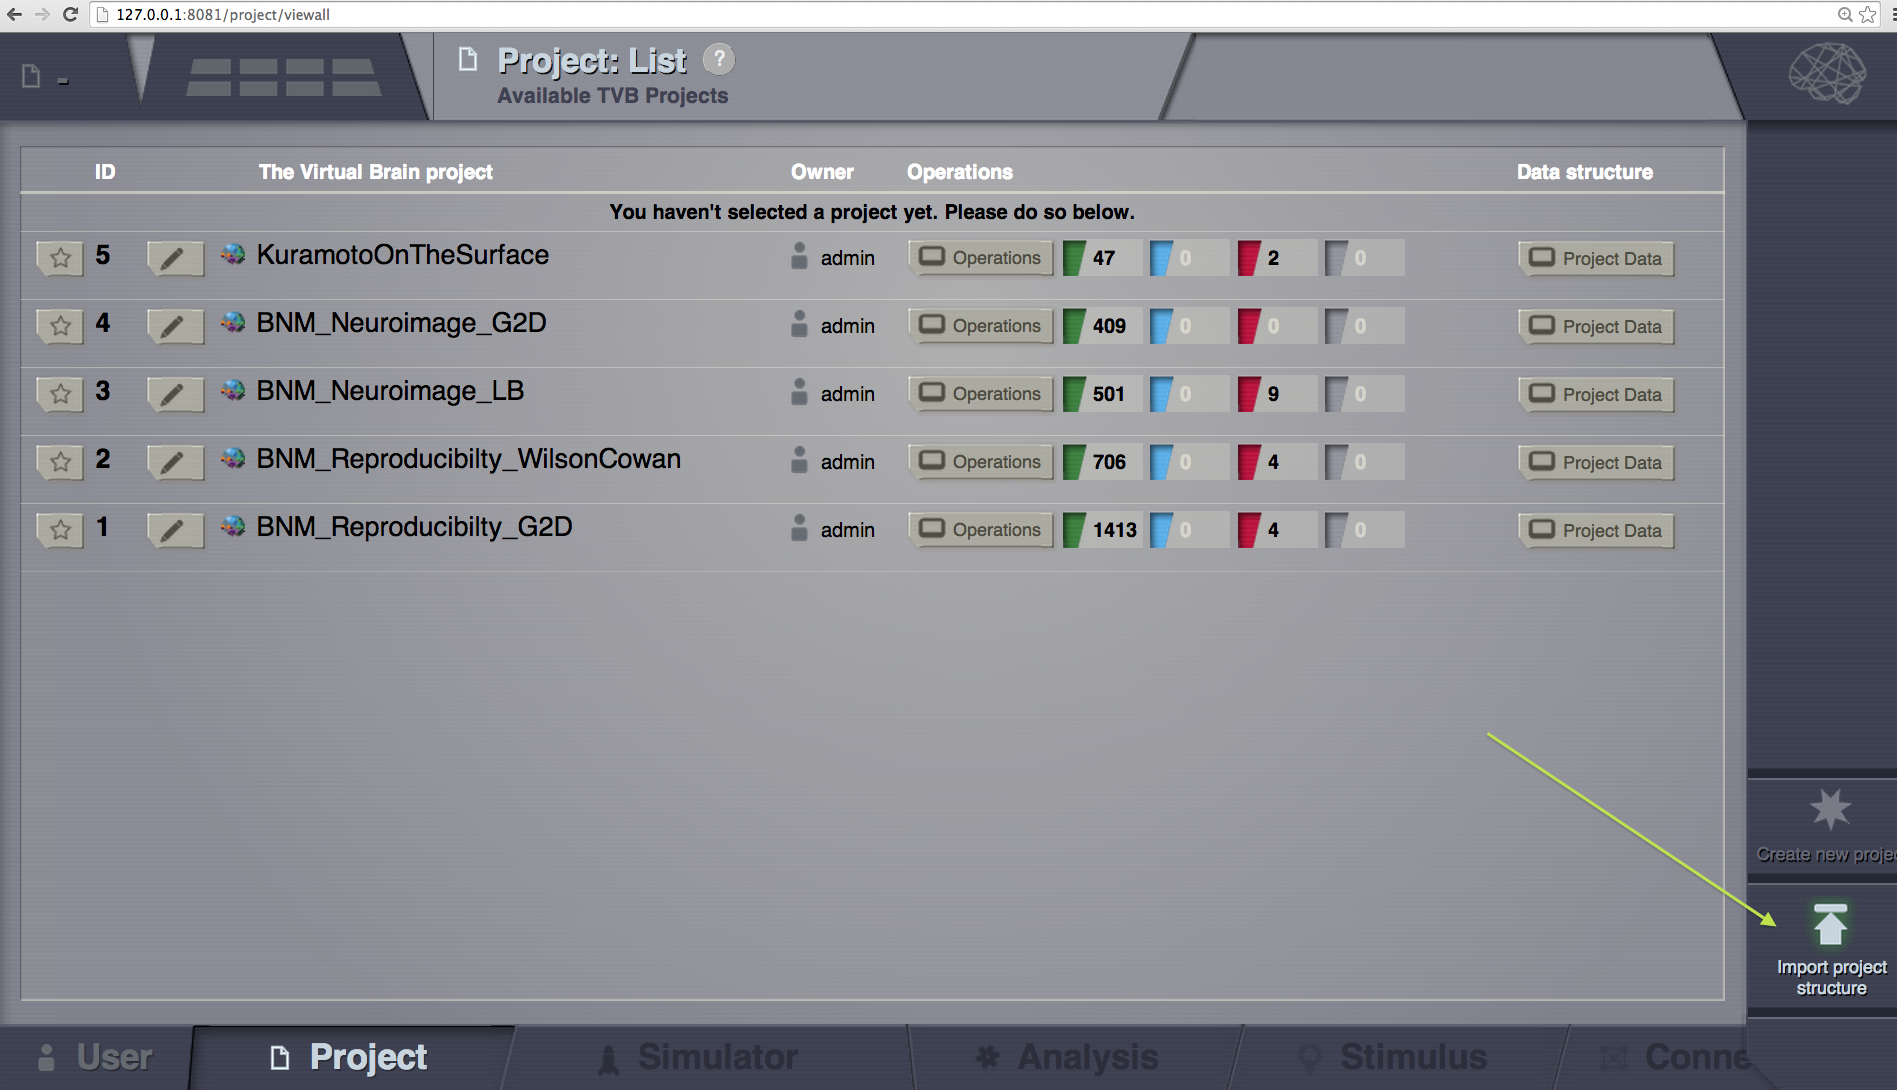
\includegraphics[width=\linewidth]{Handout_UI_ImportingProjects_Import}%
  \caption{Click on \underline{Import project structure}}%
  \label{fig:import}%
\end{figure}

\begin{figure}
  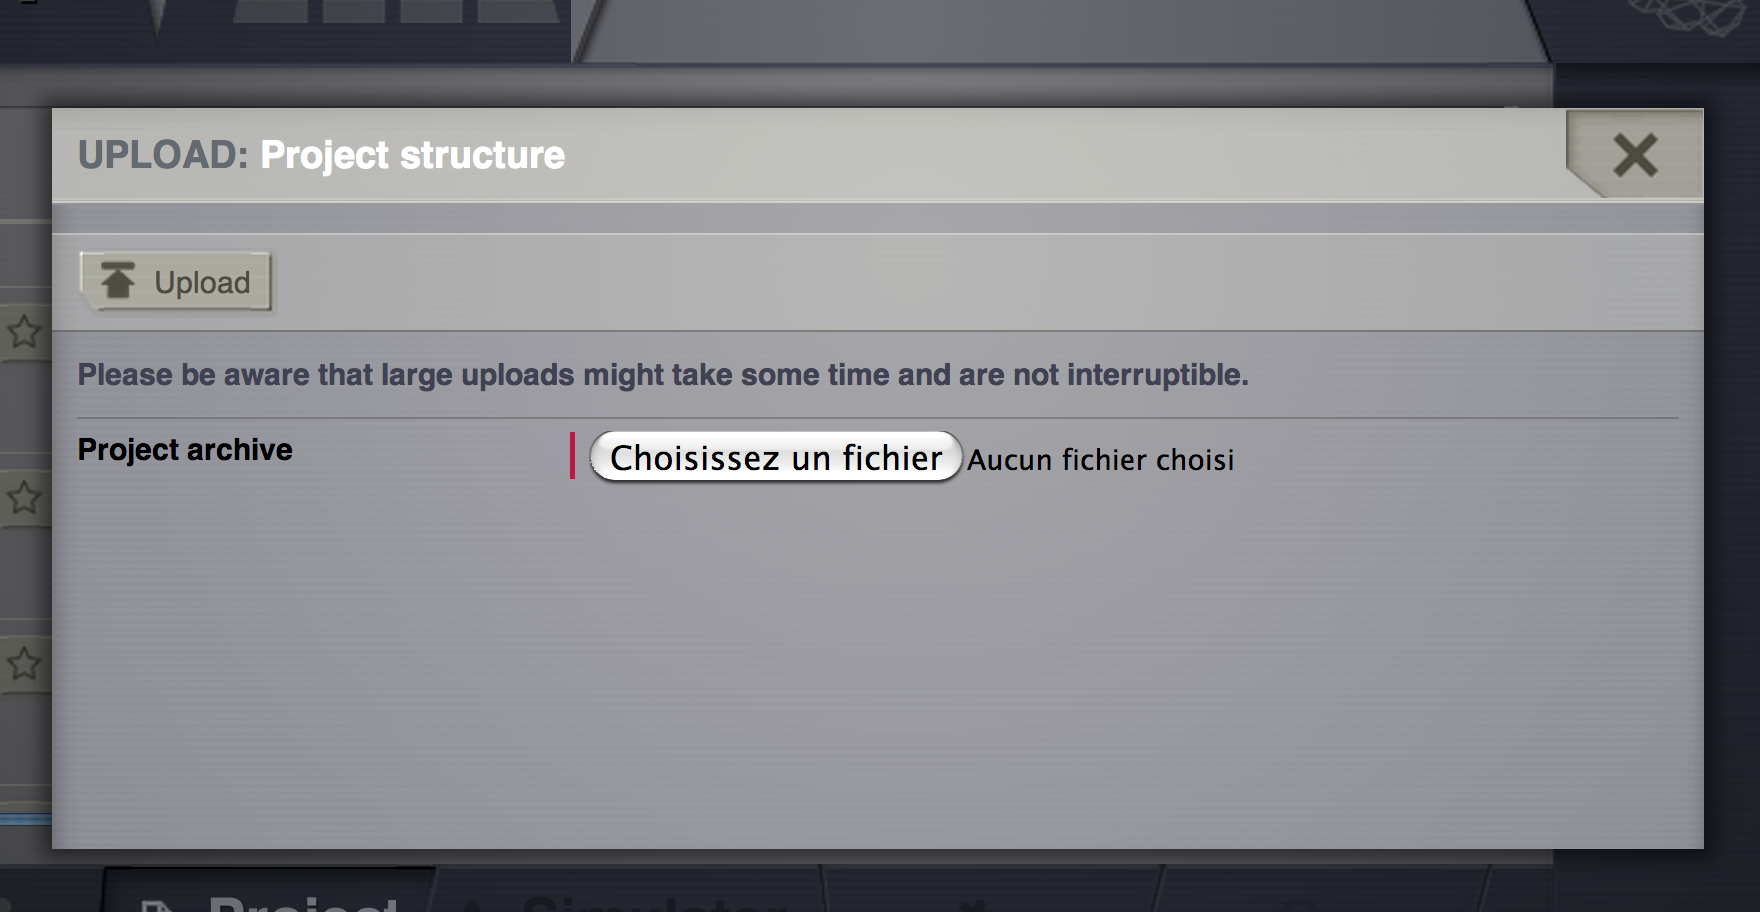
\includegraphics[width=\linewidth]{Handout_UI_ImportingProjects_ImportOverlay}%
  \caption{Click on \underline{Select files}}%
  \label{fig:importoverlay}%
\end{figure}

\begin{figure}
  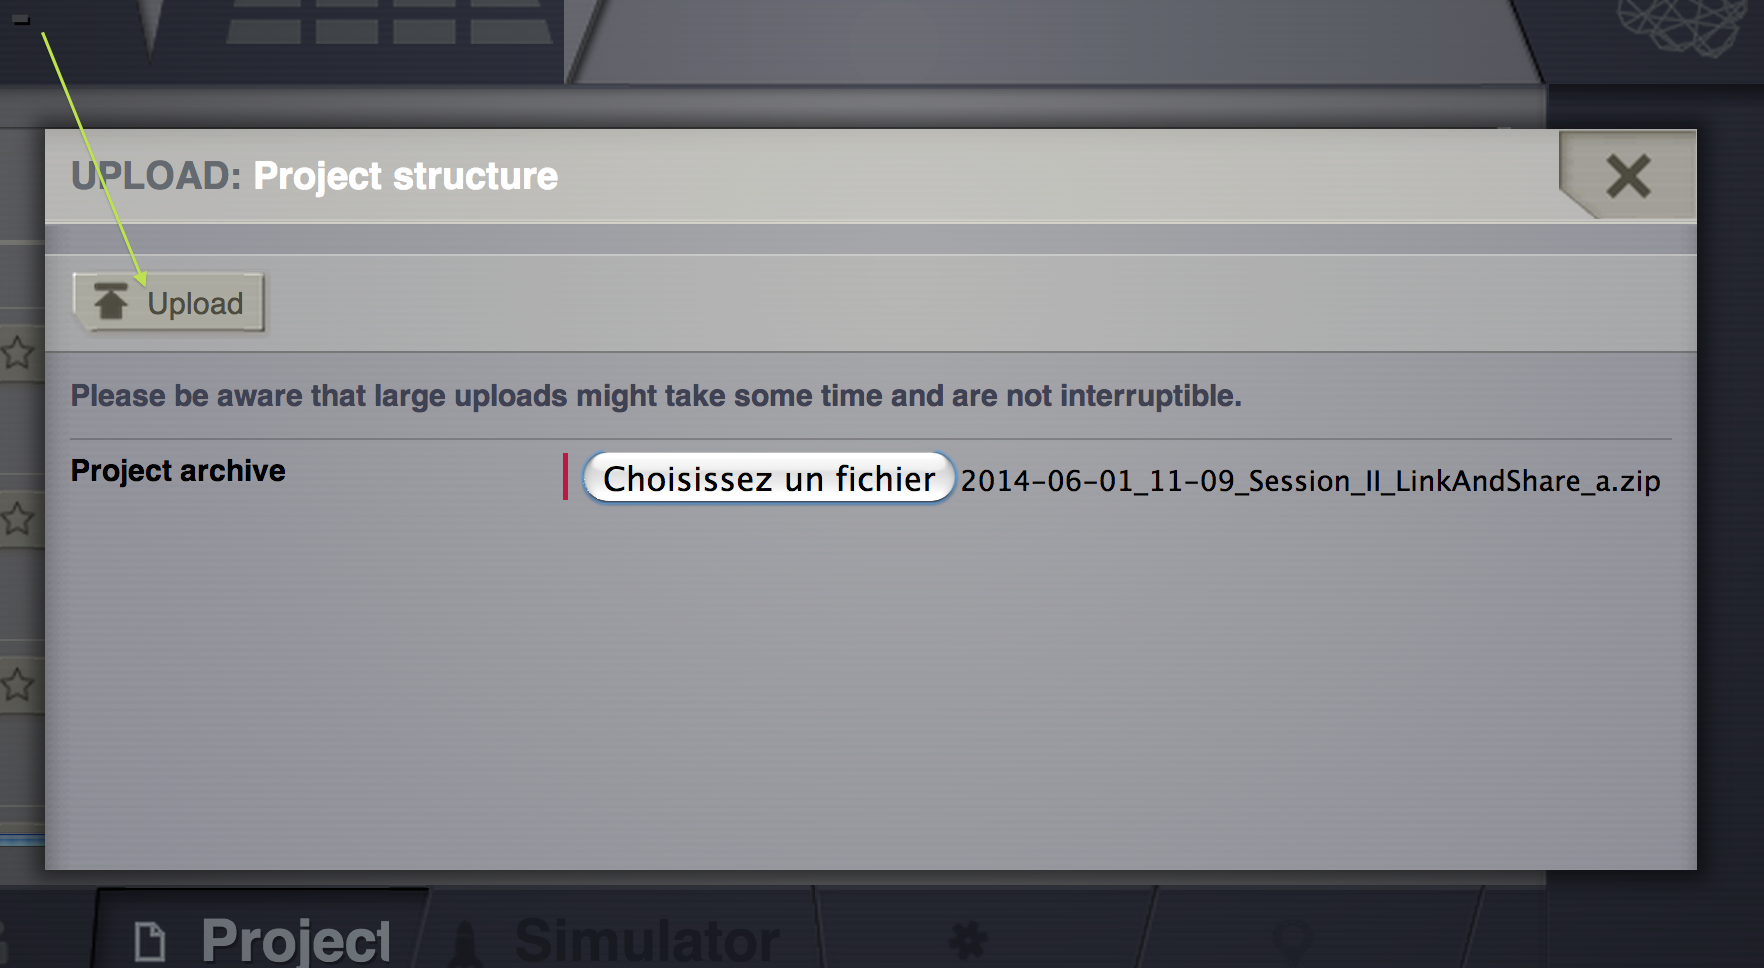
\includegraphics[width=\linewidth]{Handout_UI_ImportingProjects_Upload}%
  \caption{Upload.}%
  \label{fig:importupload}%
\end{figure}

\begin{figure}
  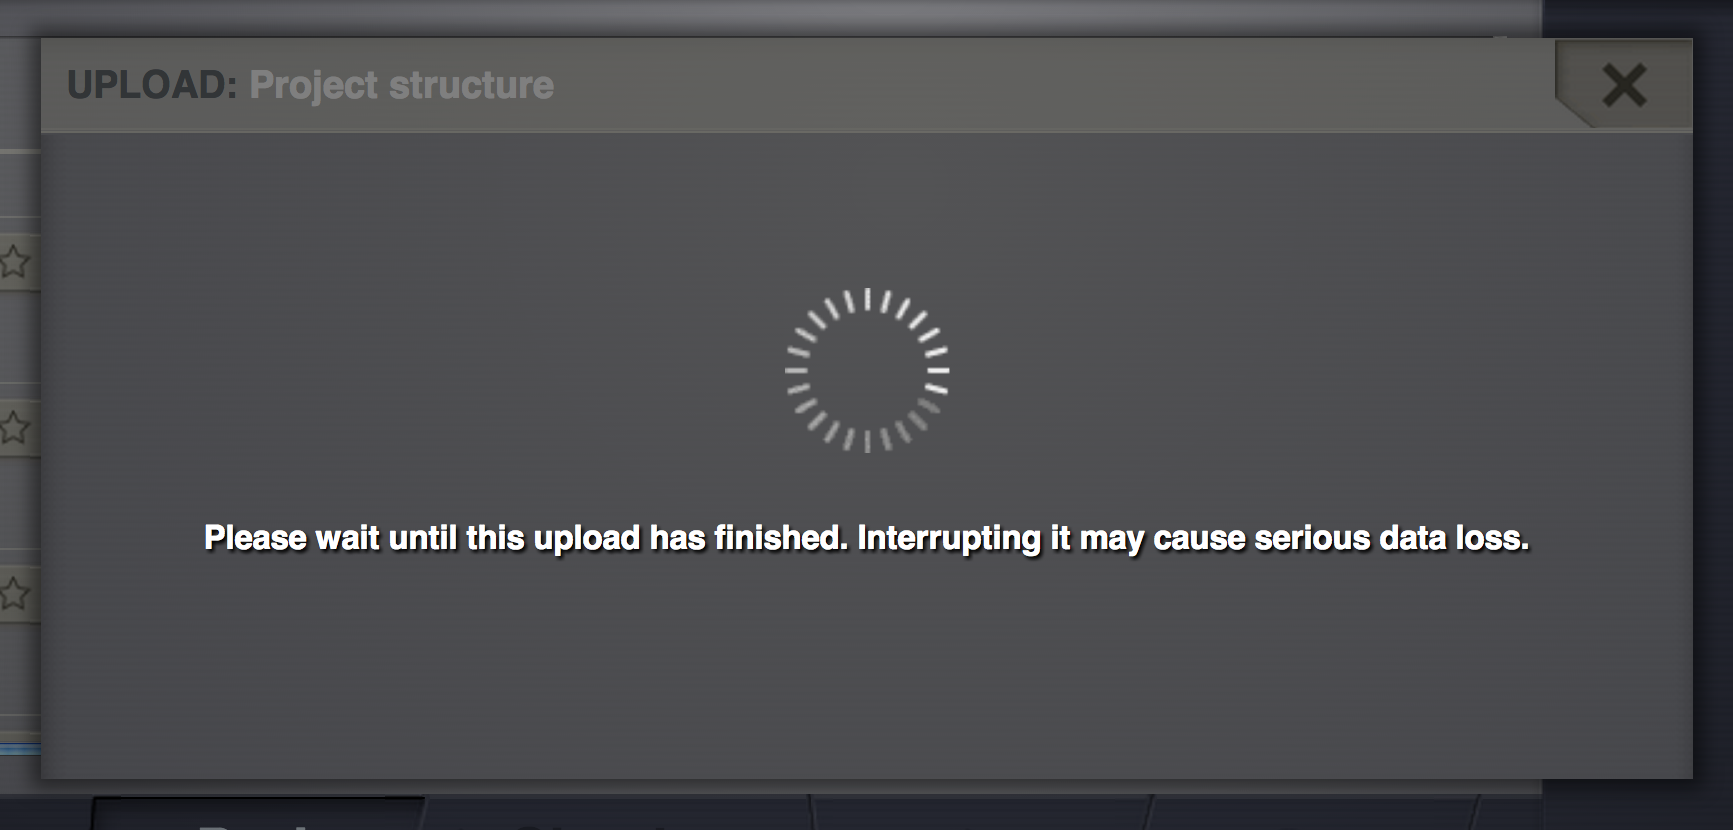
\includegraphics[width=\linewidth]{Handout_UI_ImportingProjects_Wait}%
  \caption{Be patient, it will take a few minutes.}%
  \label{fig:importwait}%
\end{figure}

\begin{figure}
  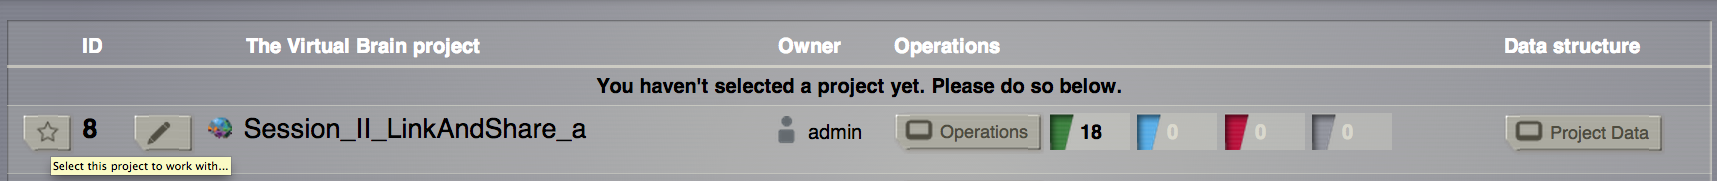
\includegraphics[width=\linewidth]{Handout_UI_ImportingProjects_Done}%
  \caption{The imported project is on the \underline{List of all projects}.}%
  \label{fig:importdone}%
\end{figure}


\newpage

\section{More Documentation}\label{sec:more-doc}
Online help is available clicking on the 
\includegraphics[width=0.05\textwidth]{butt_green_help} icons next to each entry.
For more documentation on The Virtual Brain platform, please see the following articles \citep{Sanz-Leon_2013, Woodman_2014}


\section{Support}\label{sec:support}

The official TVB webiste is \url{www.thevirtualbrain.org}.  
All the documentation and tutorials are hosted on \url{the-virtual-brain.github.io}.
You'll find our public \smallcaps{git} repository at \url{https://github.com/the-virtual-brain}. 
For questions and bug reports we have a users group \url{https://groups.google.com/forum/#!forum/tvb-users}

\bibliography{tvb_references}
\bibliographystyle{plainnat}

\end{document}